本章では,姿勢推定の従来法の説明をする.


\section{6次元物体検出}
6次元の物体検出は,3次元空間座標だけでなく物体のroll,pitch,yawの3次元姿勢情報を含んだ検出問題である.
高速に推定を行えることに加え,6次元の姿勢情報を持つ教師データがなくても学習可能な手法である.
6次元の姿勢情報を持つ教師データの代わりに,検出対象となる物体の3D CADデータを使用する.
6次元物体検出における,全体の処理の流れを図\ref{fig:2d_pose_estimation}\cite{AAE}に示す.
      \begin{figure}[htbp]
      \begin{center}
      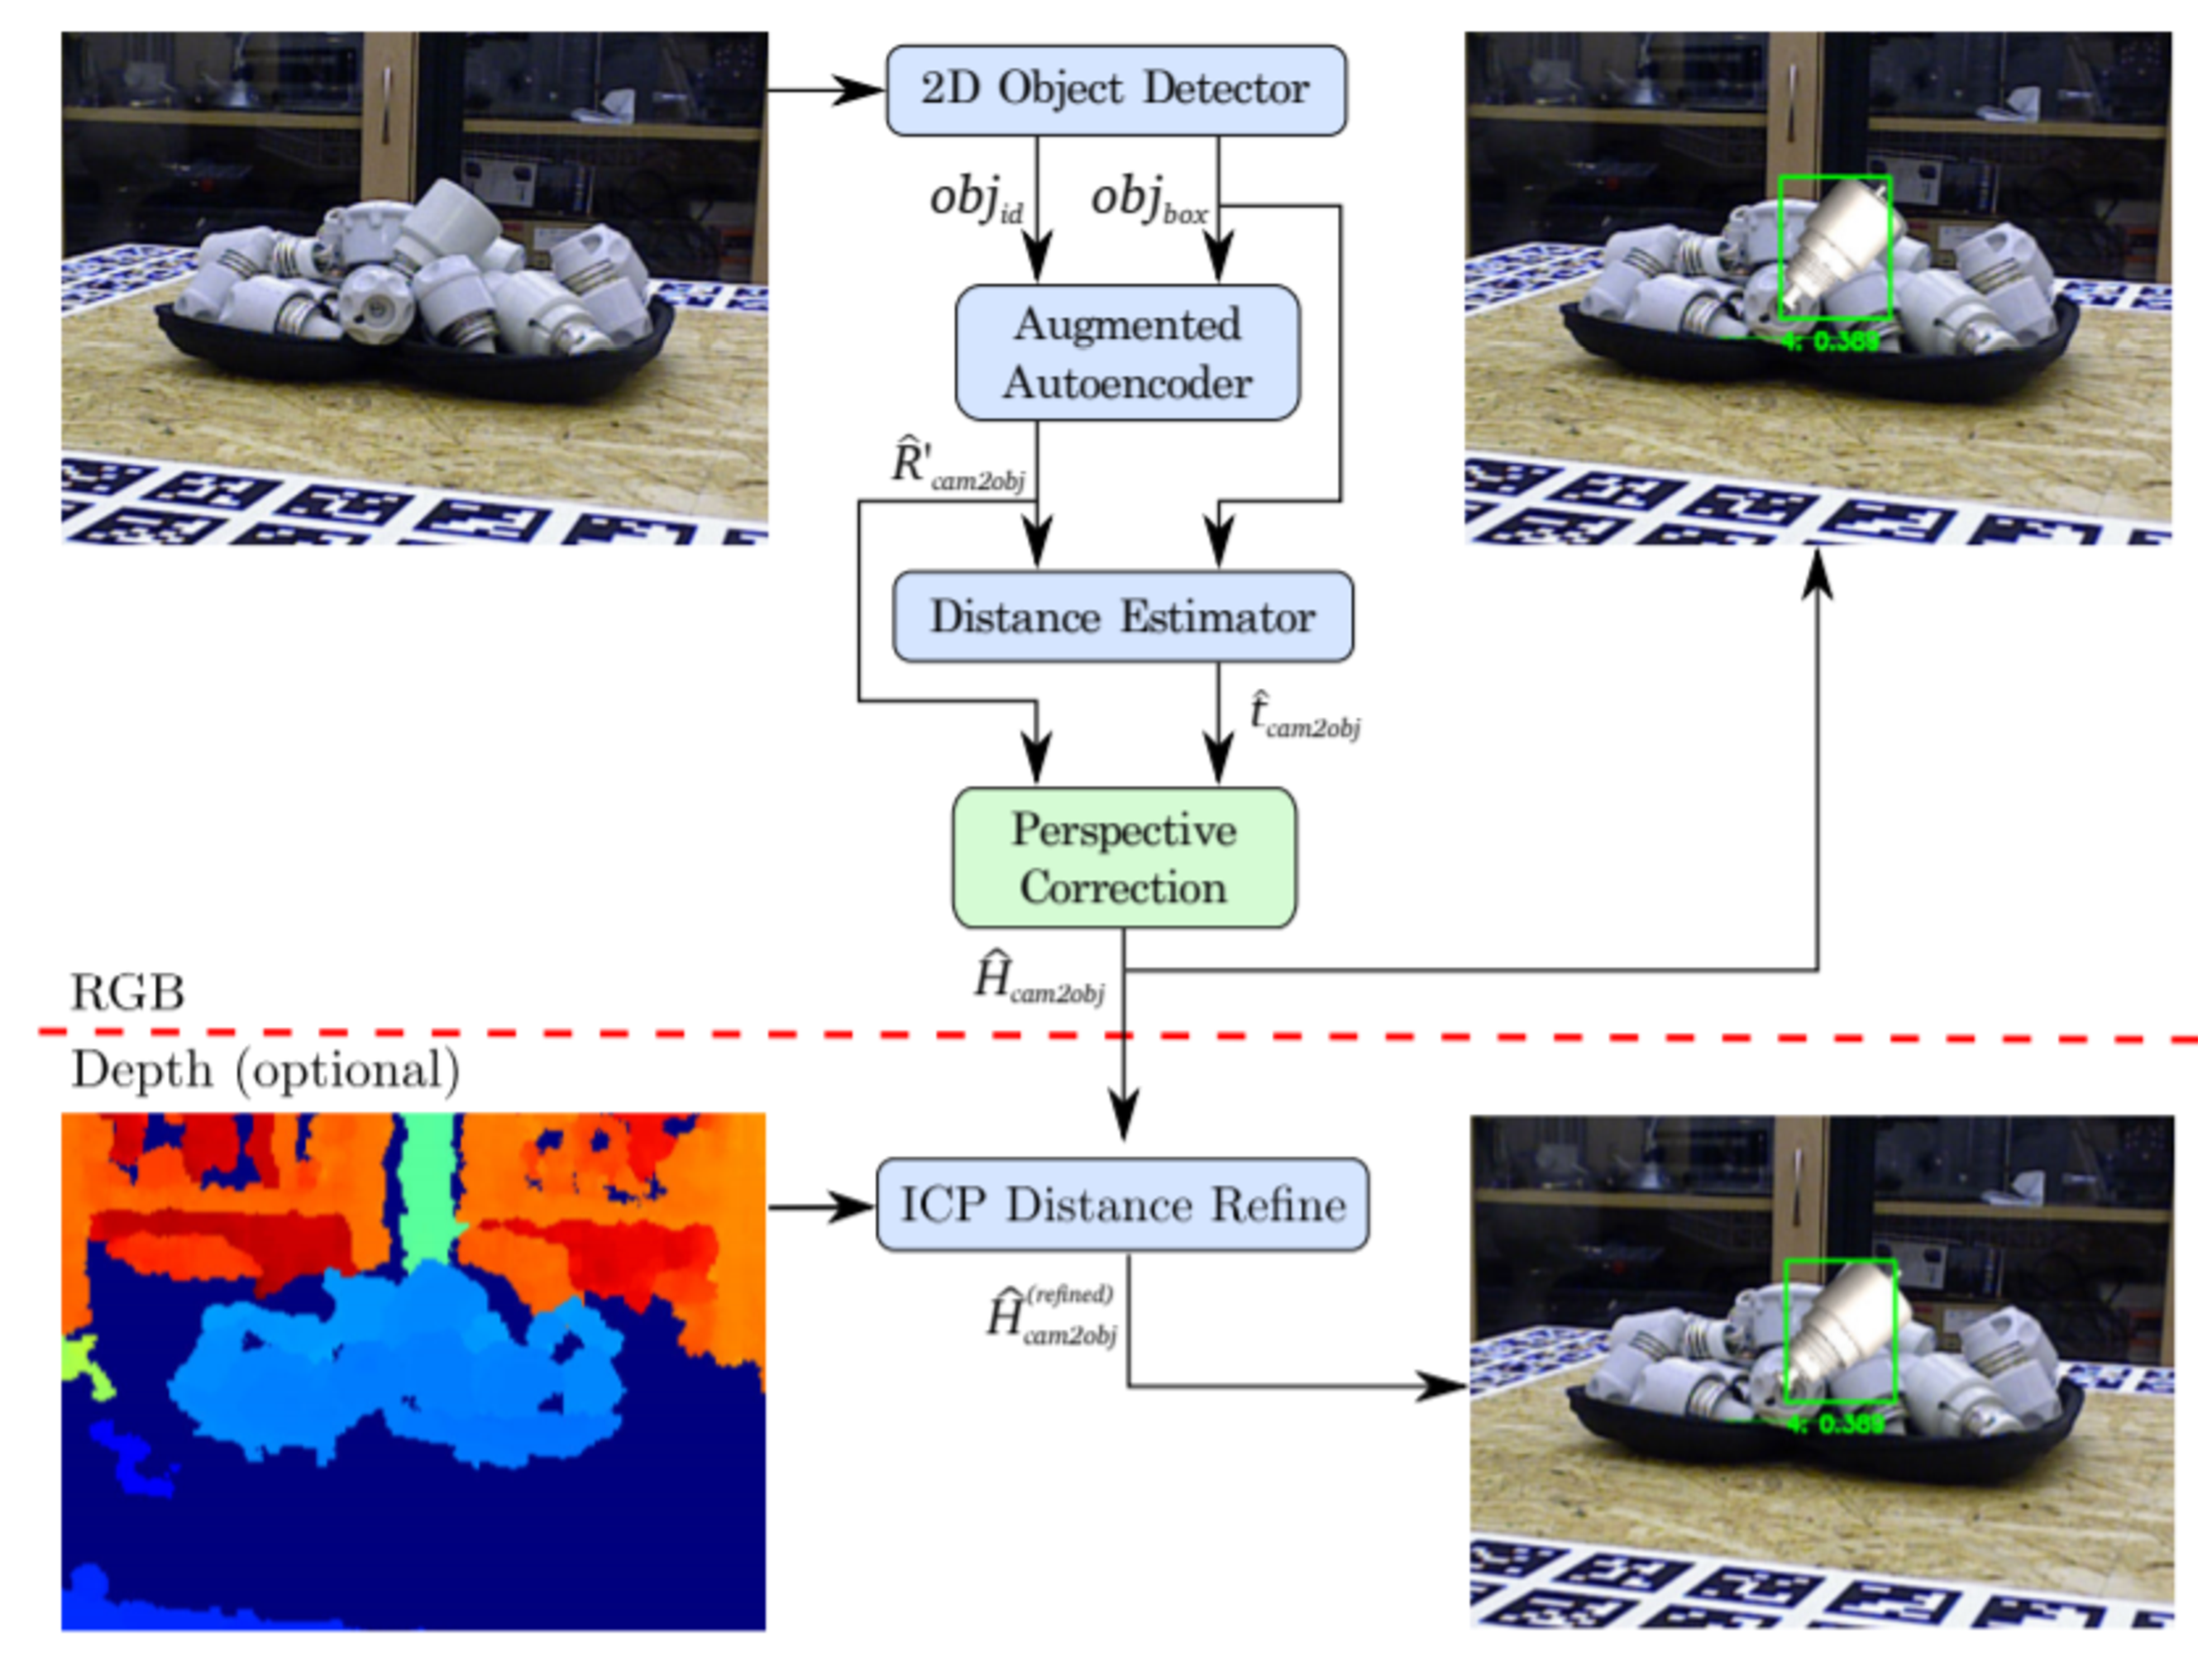
\includegraphics[width=100mm]{figure/eps/6次元推定.eps}
      \caption{6次元物体検出.}
      \label{fig:2d_pose_estimation}
      \end{center}
      \end{figure}



入力となるRGB画像に対してSSD\cite{SSD}を用いて対象物体のID,座標位置,Bounding Boxを検出する.
その後,検出されたBounding Box領域から物体の姿勢情報をAugumented Autoencoderにより取得し,推定を行う.
 


\subsection{Augumented Autoencoder}
AAEの基礎となるのがAutoencoder\cite{AE}である,オートエンコーダーは訓練データのみを使用する教師なし学習の一つである.入力データ$x_i$をエンコーダー$\phi$に入力し,デコーダ$\psi$から得られる出力$x’_i$との損失関数式(\ref{eq:polynomial2})を計算し学習を行い,データを表現する潜在変数zを獲得するためのニューラルネットワークである.潜在変数は式(\ref{eq:polynomial1})によって求められる.

\begin{eqnarray}
\label{eq:polynomial2}
l_2=  \sum_{i}\parallel{ x_i - x'_i} \parallel_2
\end{eqnarray}

\begin{eqnarray}
\label{eq:polynomial1}
( x ^ {\prime})  = (\psi \times  \phi )( x ) = \psi (z)
\end{eqnarray}



AAEでは,オートエンコーダーを発展させたノイズ除去を行い潜在変数を取得するDenoising Autoencoder\cite{DAE}が応用されている.
エンコーダーに訓練データの一部にノイズを加えた画像を入力し,ノイズなしの画像を出力できるよう,
ノイズのない訓練データとの損失関数を学習させることで,
ノイズによらない本質的な潜在表現を得ることができる方法である.

また,Domain Randomization\cite{Dm}という手法も取り入れられている.
この手法の目的は,評価時にモデルが実世界のデータに一般化できるよう,
環境ノイズを加えた3Dモデルをランダムに作成し学習を行う.
これにより物体と背景の対称性を明確にして,評価時に現実世界での推定も可能になる.

上記のDenoising AutoencoderとDomain Randomizationの手法を取り入れ応用したオートエンコーダーがAAEである.
AAEの学習を図\ref{AAEgakusyu}に示す.図\ref{AAEgakusyu}(a)の訓練データxに背景や光,遮蔽物などの環境ノイズ$f_augm$を追加した図\ref{AAEgakusyu}(b)の画像x''を入力し,環境ノイズなしの図\ref{AAEgakusyu}(c)の画像x'を出力するように
xとx"損失関数を計算し学習を行う.データを表現する潜在変数を式(\ref{eq:polynomial3})によって獲得する手法である.

      \begin{figure}[htbp]
      \begin{center}
      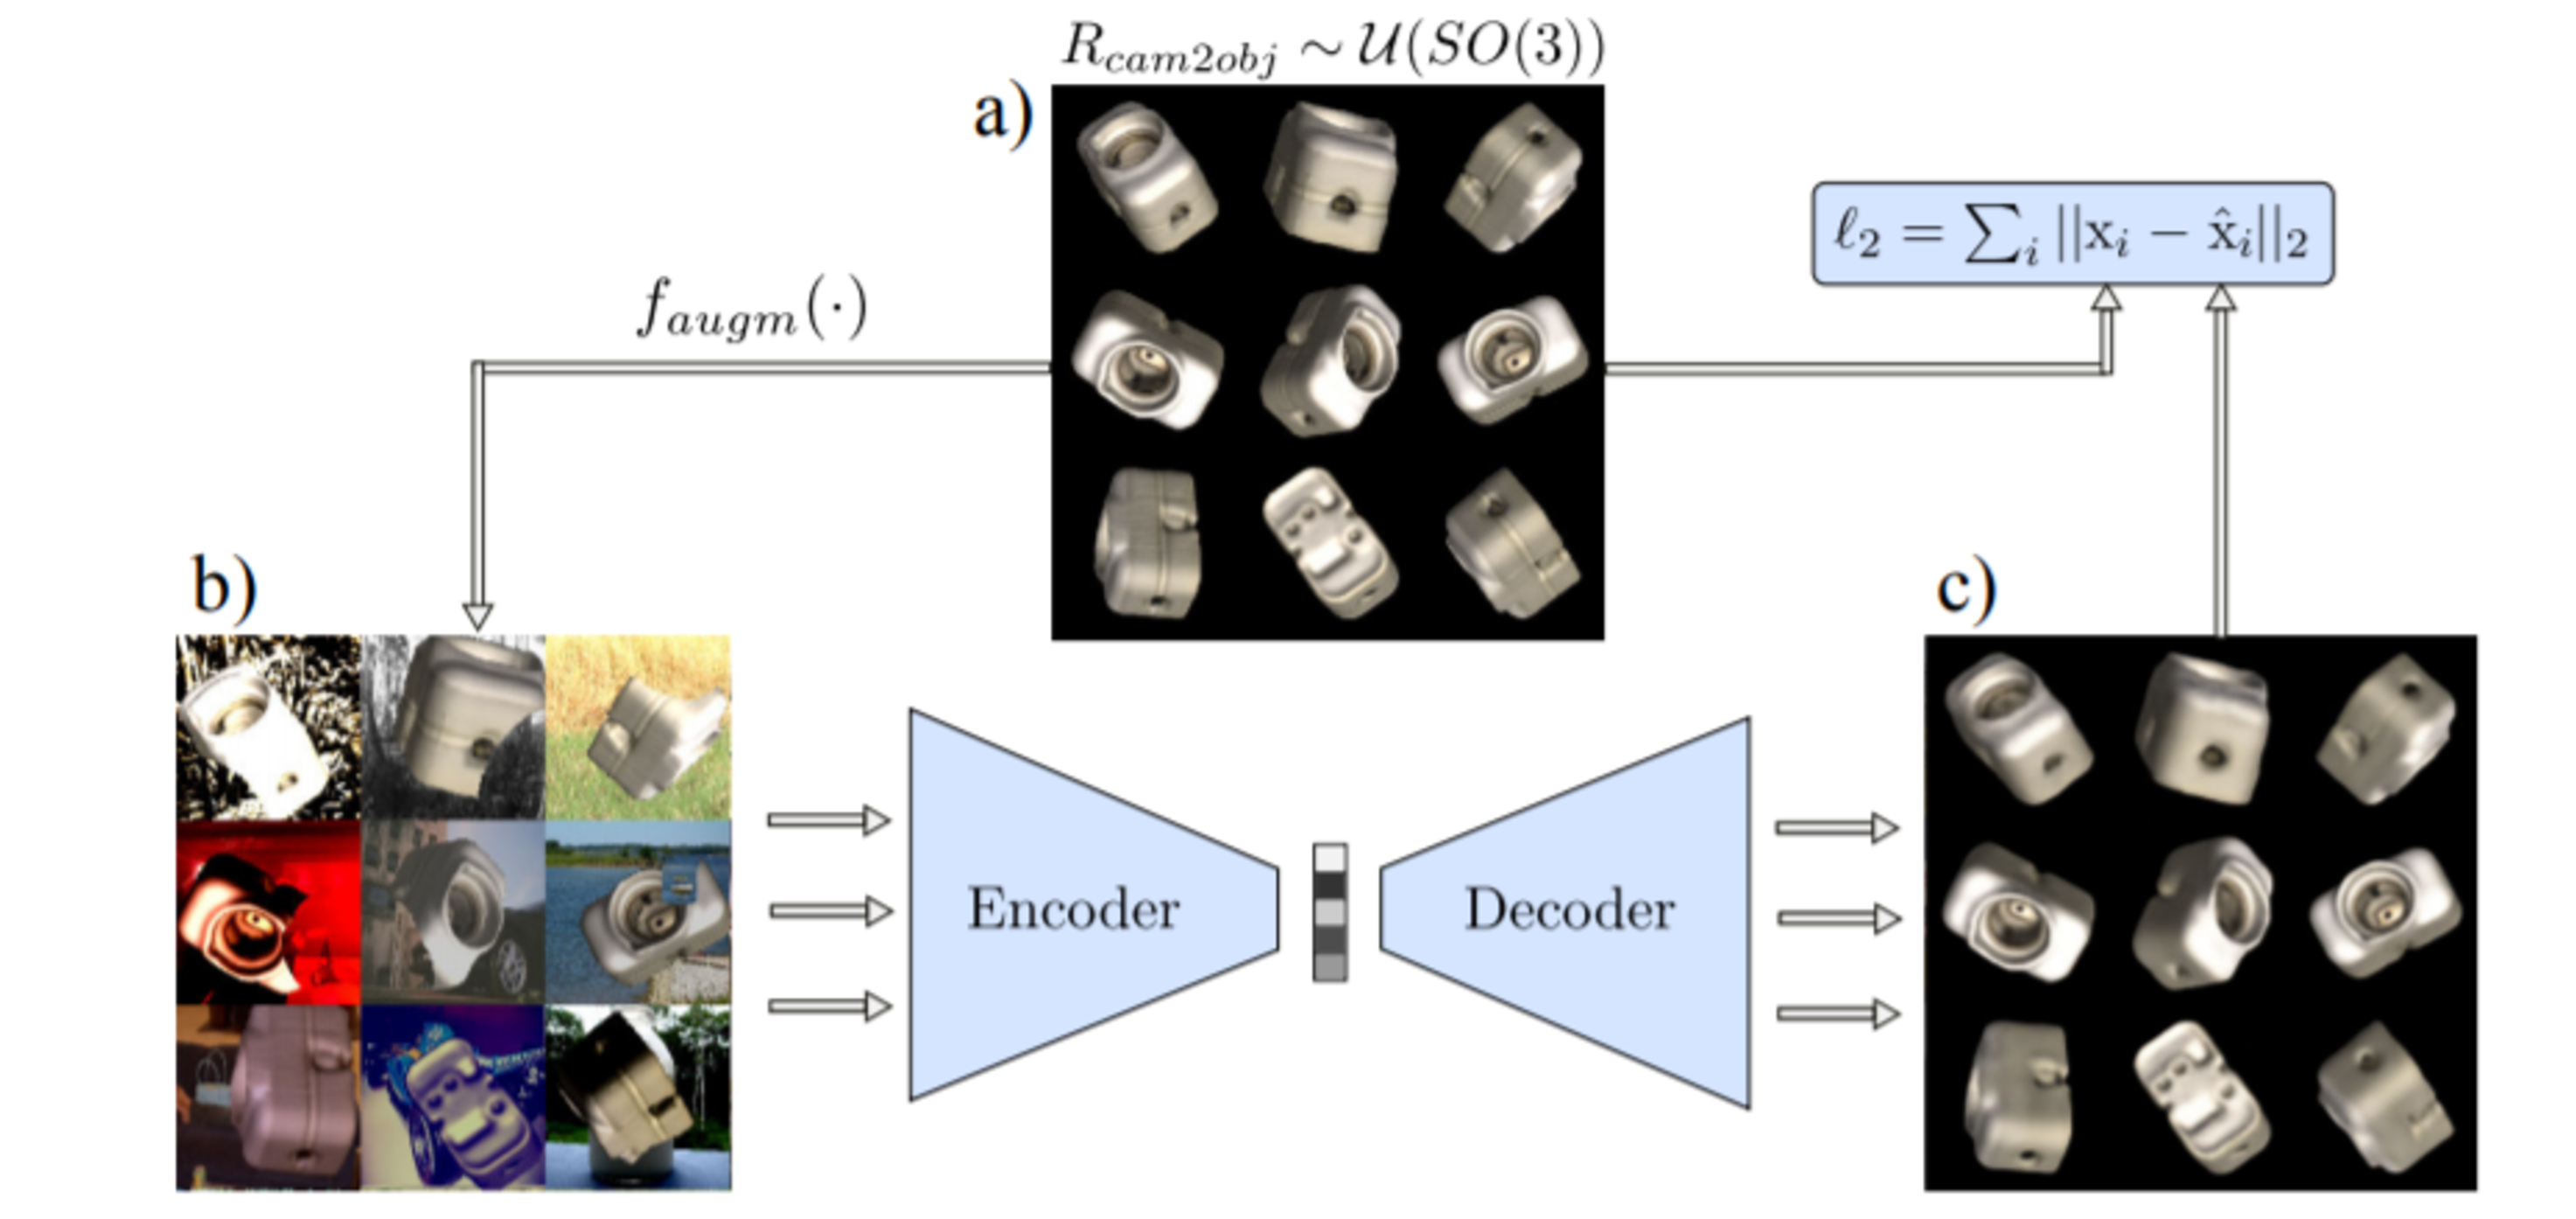
\includegraphics[width=110mm]{figure/eps/AAEの学習.eps}
      \caption{AAEの学習\cite{AAE}.}
      \label{AAEgakusyu}
      \end{center}
      \end{figure}

\begin{eqnarray}
\label{eq:polynomial3}
x ' = (\psi \times  \phi \times f_{augm} )( x ) = (\psi \times \phi) (x'') = \psi (z)
\end{eqnarray}


AAEのネットワークを図\ref{netwa}に示す.入力出力はチャンネル数3の画像サイズ128$\times$128のカラー画像を使用する.

      \begin{figure}[htbp]
      \begin{center}
      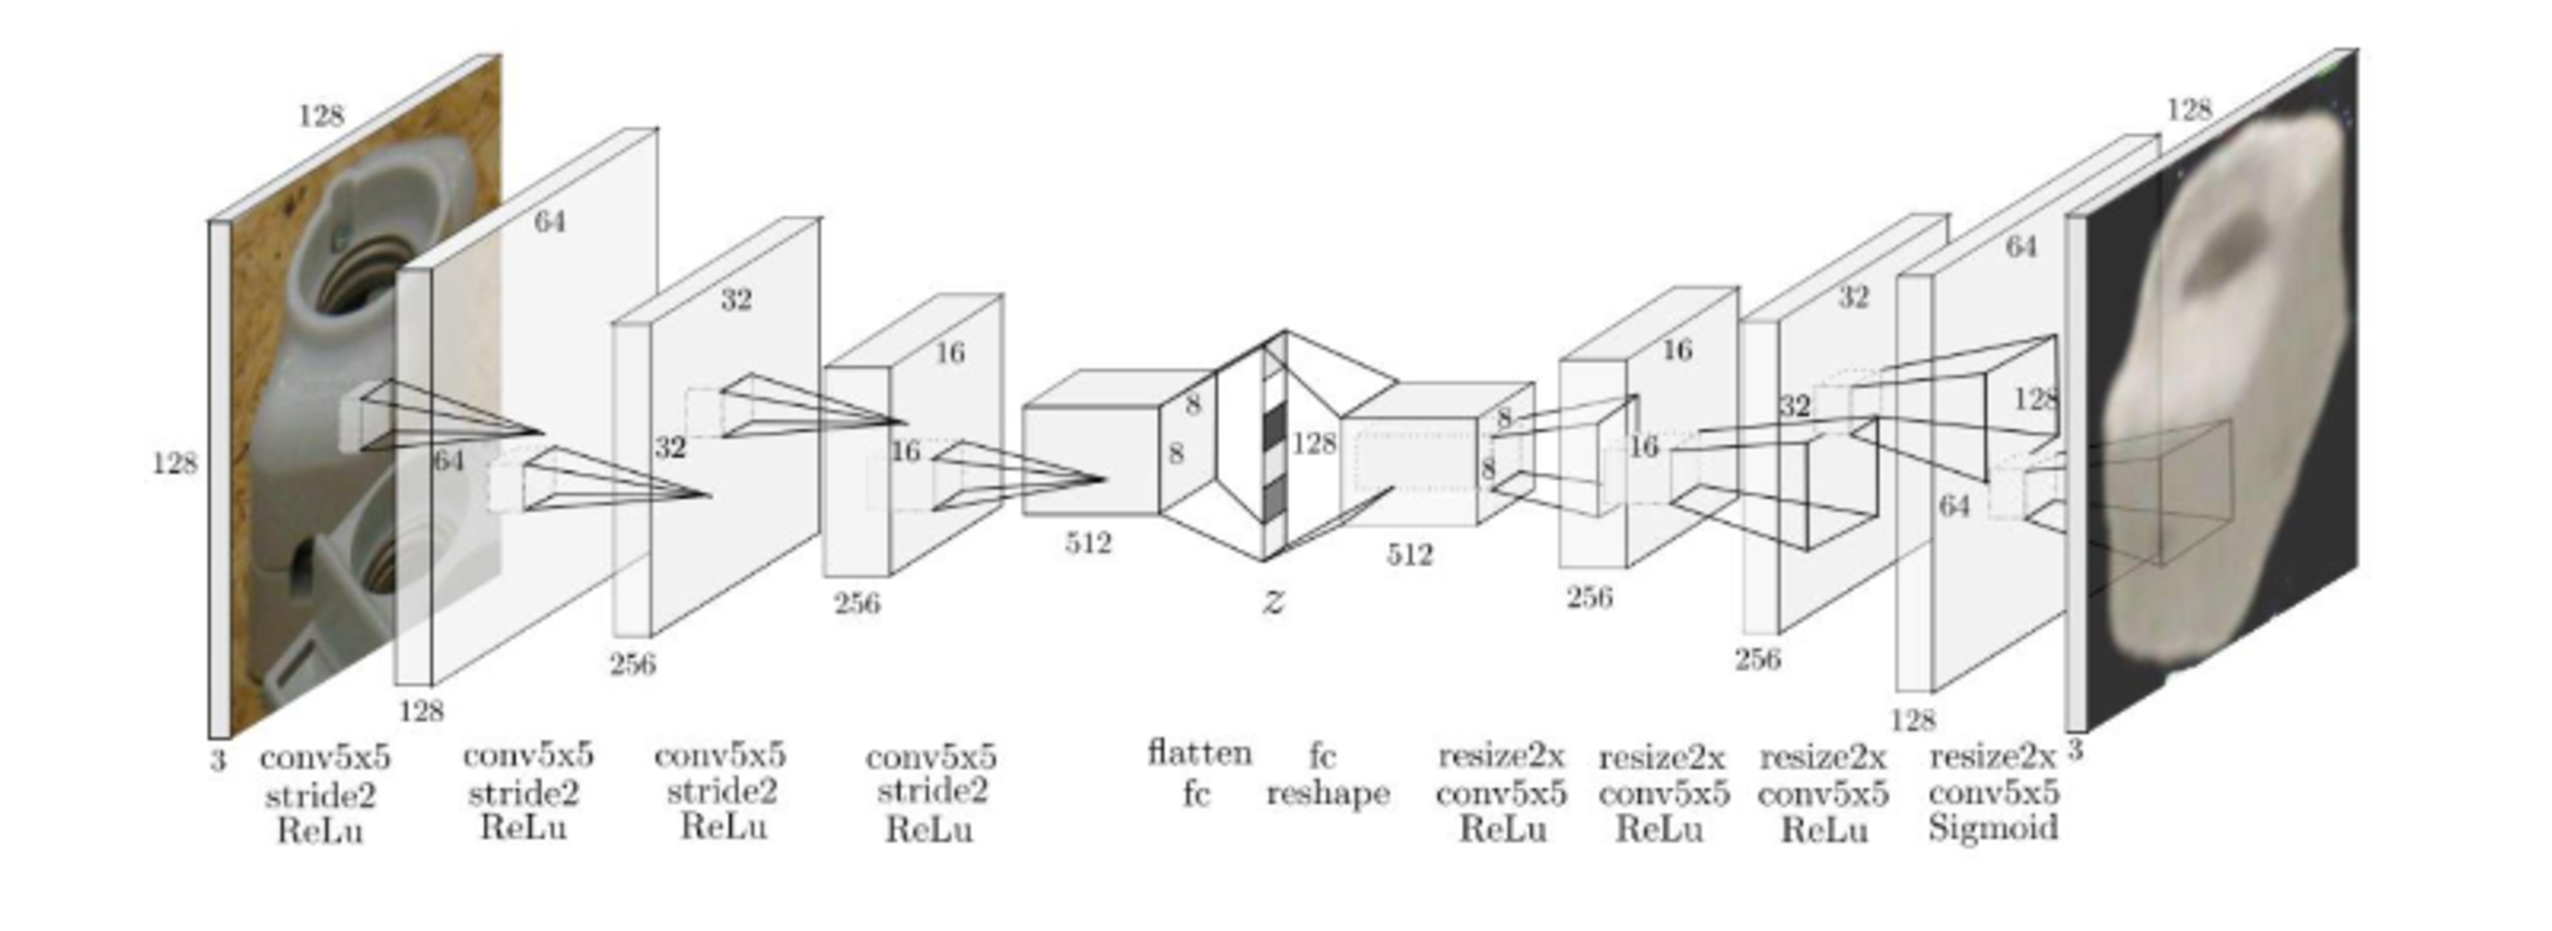
\includegraphics[width=120mm]{figure/eps/ネットワーク.eps}
      \caption{AAEのネットワーク\cite{AAE}.}
      \label{netwa}
      \end{center}
      \end{figure}





\subsection{AAEを用いた姿勢推定}


AAEによって求められる潜在変数を元に姿勢推定を行う.
推定対象となる物体の3Dモデルを作成し,3Dモデル物体を回転させ92232個の姿勢をAAEにかけ潜在変数を生成し92232個分の姿勢情報を持つ潜在変数を記録していく.
記録されている姿勢情報が既知となっている潜在変数$ z_i $と推定したい画像から新たに得た潜在変数$z_{test}$のコサイン類似度を式(\ref{cos})用いて比較し
最も近い潜在変数を持つ姿勢情報を推定姿勢として決定する.

\begin{eqnarray}
\label{cos}
cos_i = \frac {z_i \times z_{test}}{|z_i||z_{test}|}
\end{eqnarray}

